% ============================================== %

%%%%%%%%%%%%%%%%%%%%%%%%%%%%%%%%%%%%%%%%%%%%%%%%%%
%%%			  10 Trabalho Prático 10		   %%%
%%%%%%%%%%%%%%%%%%%%%%%%%%%%%%%%%%%%%%%%%%%%%%%%%%

% ============================================== %

\section{Trabalho Prático 10}

Ler e resumir o artigo:

\begin{center}
	YANG, Y. -B.; SHIEH, M. -S. (1990)

	\textit{"Solution method for nonlinear problems with multiple critical points."}

	AIAA Journal, V. 28, p. 2110-2116.
\end{center}


% ================ Resolução TP-10 ================
\begin{textocaixa}

\hspace{10mm}
O artigo de Yang e Shieh (1990) propõe um método aprimorado para a solução de problemas
não-lineares geométricos com múltiplos pontos críticos, denominado \textbf{Método de
Controle de Deslocamento Generalizado} (\textit{Generalized Displacement Control Method} --
GDC). O desenvolvimento se insere no contexto de análises estruturais nas quais a curva
carga-deslocamento exibe \textit{pontos limite} (onde a rigidez tangente se anula e o caminho
de equilíbrio muda de estável para instável) e \textit{pontos de retrocesso}
(\textit{snap-back points}), onde o próprio deslocamento de controle inverte de sentido.

\subsection*{Formulação no Espaço de Dimensão $N+1$}

A equação matricial que governa a $j$-ésima iteração do $i$-ésimo incremento de um sistema
com $N$ graus de liberdade é escrita como:

\begin{equation}
	[K]^{i}_{j-1}\{u\}^{i}_{j} = \lambda^{i}_{j}\{P\} + \{R\}^{i}_{j-1}
\end{equation}

Onde $[K]$ é a matriz de rigidez tangente, $\{u\}$ o vetor de incremento de deslocamentos,
$\{P\}$ o vetor de carga de referência, $\lambda$ o parâmetro de incremento de carga e
$\{R\}$ o vetor de forças desequilibradas. Como ambos $\{u\}$ e $\lambda$ são incógnitas,
uma equação de restrição adicional é necessária:

\begin{equation}
	\langle C \rangle \{u\}^{i}_{j} + k\,\lambda^{i}_{j} = H^{i}_{j}
	\label{eq:restricao_tp10}
\end{equation}

A seleção adequada das constantes $\langle C \rangle$, $k$ e $H^i_j$ na
\autoref{eq:restricao_tp10} é o ponto central que distingue os diferentes métodos de solução.
Os autores mostram que, para garantir estabilidade numérica, o parâmetro de incremento de
carga $\lambda^i_j$ deve permanecer limitado durante toda a análise. Por decomposição da
matriz de rigidez generalizada $[\bar{K}_1]$ no espaço $N+1$, obtém-se a expressão geral:

\begin{equation}
	\lambda^{i}_{j} = \frac{H^{i}_{j} - \lambda^{i}_{1}
					       \langle u_1 \rangle^{i-1}_{1}\{u_2\}^{i}_{j}}
						   {\lambda^{i}_{1}\langle u_1 \rangle^{i-1}_{1}\{u_1\}^{i}_{j}}
	\label{eq:lambda_tp10}
\end{equation}

Na qual $\{u_1\}^{i-1}_1$ é o vetor de deslocamentos resultante da primeira iteração do
último passo incremental.

\subsection*{Avaliação dos Métodos Existentes}

Os autores utilizam a Equação~\eqref{eq:lambda_tp10} como critério analítico para avaliar os
métodos clássicos:

\begin{itemize}
	\item \textbf{Newton-Raphson:} mantém $\lambda$ limitado nos passos iterativos, porém o
	incremento de deslocamento $\{u\}_j$ pode divergir próximo a pontos limite, pois
	$\det[K] \to 0$ nesses pontos.

	\item \textbf{Controle de Deslocamento:} contorna os pontos limite com sucesso, mas
	falha nos pontos de retrocesso: quando o deslocamento de controle $u^c$ tende a zero,
	$\lambda^i_j \to \infty$.

	\item \textbf{Comprimento de Arco (\textit{Arc-Length}):} pode gerar sinais incorretos
	para $\lambda$ nas proximidades de pontos de retrocesso com gradientes acentuados, além
	de não fornecer de forma automática a informação necessária para inverter a direção de
	carregamento.

	\item \textbf{Controle de Trabalho:} baseado no Parâmetro de Rigidez Atual (CSP --
	\textit{Current Stiffness Parameter}), que apresenta descontinuidades próximas a pontos
	de retrocesso e muda de sinal tanto em pontos limite quanto em pontos de retrocesso,
	sendo um indicador inadequado para a inversão de direção de carregamento.
\end{itemize}

\subsection*{Método Proposto: Controle de Deslocamento Generalizado}

Adotando $k = 0$ e $\langle C \rangle = \lambda^{i}_{1}\langle u_1 \rangle^{i-1}_{1}$ na
equação de restrição geral, obtém-se, para o passo incremental ($j=1$):

\begin{equation}
	\lambda^{i}_{1} = \lambda^{1}_{1}\left(\frac{\langle u_1 \rangle^{1}_{1}\{u_1\}^{1}_{1}}
								 {\langle u_1 \rangle^{i-1}_{1}\{u_1\}^{i}_{1}}\right)^{1/2}
	= \lambda^{1}_{1}\,(\text{GSP})^{1/2}
\end{equation}

E, para as iterações subsequentes ($j \geq 2$):

\begin{equation}
	\lambda^{i}_{j} = -\frac{\langle u_1 \rangle^{i-1}_{1}\{u_2\}^{i}_{j}}
							{\langle u_1 \rangle^{i-1}_{1}\{u_1\}^{i}_{j}}
\end{equation}

O \textbf{Parâmetro de Rigidez Generalizado} (GSP --
\textit{Generalized Stiffness Parameter}) é definido como:

\begin{equation}
	\text{GSP} = \frac{\langle u_1 \rangle^{1}_{1}\{u_1\}^{1}_{1}}
					  {\langle u_1 \rangle^{i-1}_{1}\{u_1\}^{i}_{1}}
\end{equation}

Onde o numerador representa os deslocamentos do primeiro passo e o denominador os do passo
atual. O GSP apresenta as seguintes propriedades fundamentais:

\begin{enumerate}
	\item Inicia com valor unitário e é nulo nos pontos limite, tal como o CSP;
	\item É negativo \underline{apenas} para os passos imediatamente após os pontos limite
	-- ao contrário do CSP, que muda de sinal também nos pontos de retrocesso --, tornando-o
	um indicador confiável e exclusivo para a inversão da direção de carregamento;
	\item Não apresenta descontinuidades numéricas nas proximidades de pontos de retrocesso,
	ao contrário do CSP, que exibe variações abruptas nessas regiões.
\end{enumerate}

\subsection*{Algoritmo}

O procedimento numérico do GDC pode ser sintetizado nas seguintes etapas:

\begin{enumerate}
	\item Definir o incremento de carga básico $\lambda^{1}_{1}$ para o início;
	\item Para a \textbf{primeira iteração} ($j = 1$) de cada passo $i$: montar
	$[K]^{i}_{0}$; resolver a equação de equilíbrio para $\{u_1\}^{i}_{1}$; calcular o GSP
	(para $i \geq 2$) e determinar $\lambda^{i}_{1}$; verificar o sinal do GSP -- se
	negativo, multiplicar $\lambda^{i}_{1}$ por $-1$ para inverter a direção de carregamento;
	\item Para \textbf{iterações subsequentes} ($j \geq 2$): calcular as forças
	desequilibradas; resolver os sistemas para $\{u_1\}^{i}_{j}$ e $\{u_2\}^{i}_{j}$;
	determinar $\lambda^{i}_{j}$ e atualizar $\{u\}^{i}_{j}$;
	\item Atualizar forças internas, nível de carregamento e geometria;
	\item Repetir até atingir a convergência e, se o carregamento total não exceder o
	máximo, avançar ao próximo incremento.
\end{enumerate}

\subsection*{Exemplos Numéricos}

Os autores validam o GDC em dois exemplos de referência:

\textbf{Exemplo 1 -- Treliça de von Mises}

\begin{figure}[H]
	\centering
	\caption{Treliça de dois membros.}
	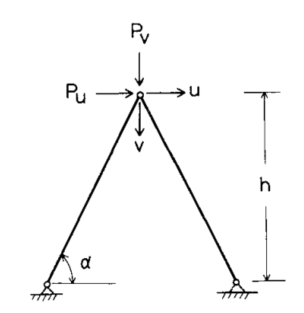
\includegraphics[
		width=0.3\textwidth
	]{figuras/TP10-ex1.png}
	\caption*{Fonte: Adaptado de YANG, Y. -B.; SHIEH, M. -S. (1990)}
	\label{fig:TP10-ex1}
\end{figure}

Para dois casos de carregamento (carga
horizontal como imperfeição: $P_u = 0{,}05\,P_v$; e carga vertical como imperfeição:
$P_v = 0{,}05\,P_u$), os resultados mostram curvas do tipo laço com quatro pontos limite
e dois pontos de retrocesso. O GDC rastreia o caminho completo de equilíbrio com sucesso,
invertendo automaticamente a direção de carregamento nos pontos limite. O GSP exibe
comportamento suave ao longo de toda a trajetória, enquanto o CSP apresenta descontinuidades
acentuadas nos pontos de retrocesso.

\begin{figure}[H]
	\centering
	\caption{Resultados gerais do Exemplo 1 para o primeiro caso de carregamento.}
	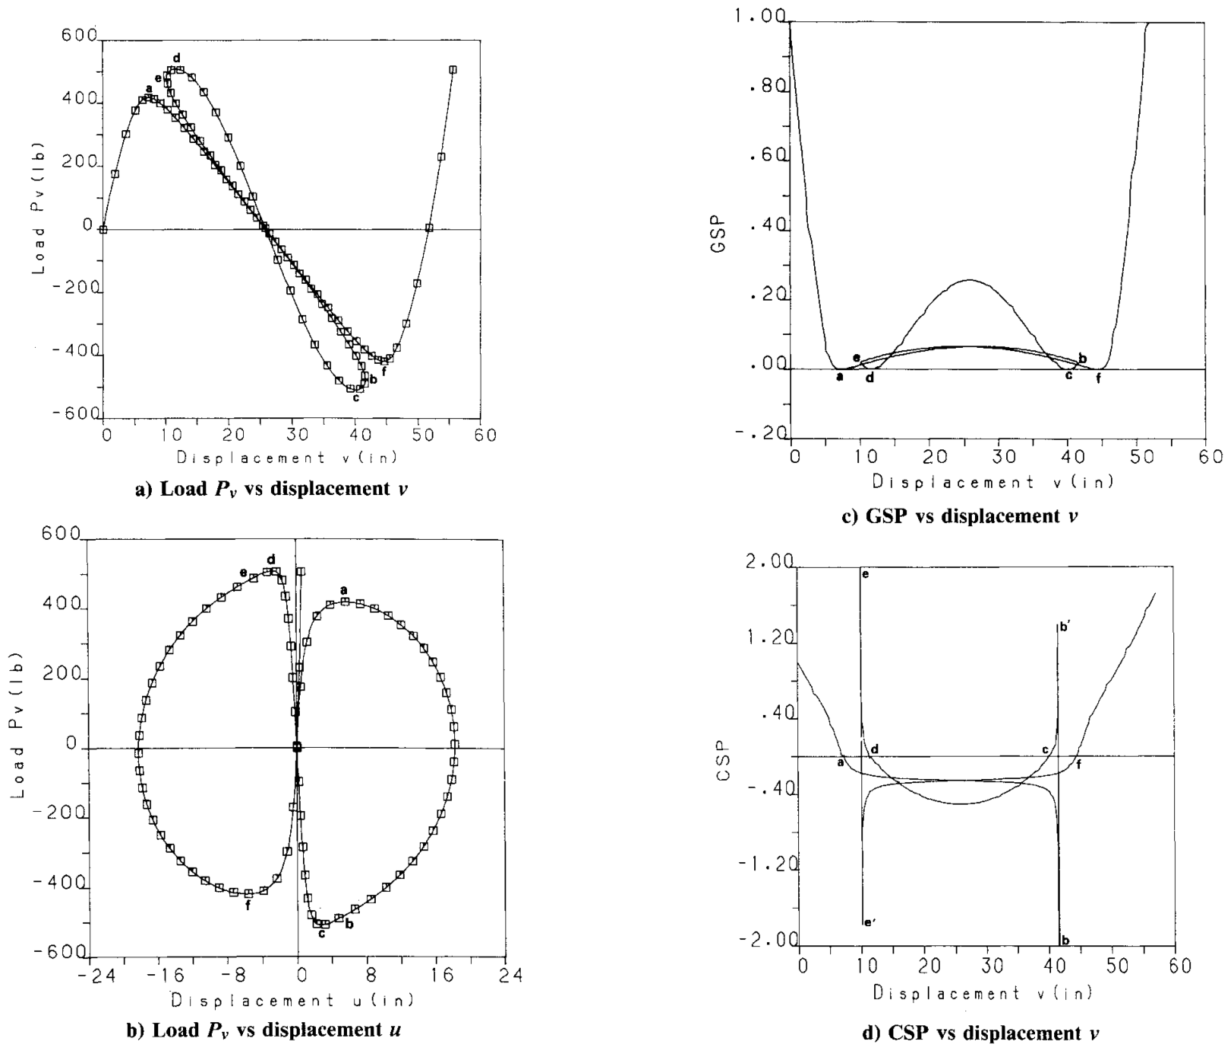
\includegraphics[
		width=\textwidth
	]{figuras/TP10-ex1_result1.png}
	\caption*{Fonte: Adaptado de YANG, Y. -B.; SHIEH, M. -S. (1990)}
	\label{fig:TP10-ex1_result1}
\end{figure}

\begin{figure}[H]
	\centering
	\caption{Resultados gerais do Exemplo 1 para o segundo caso de carregamento.}
	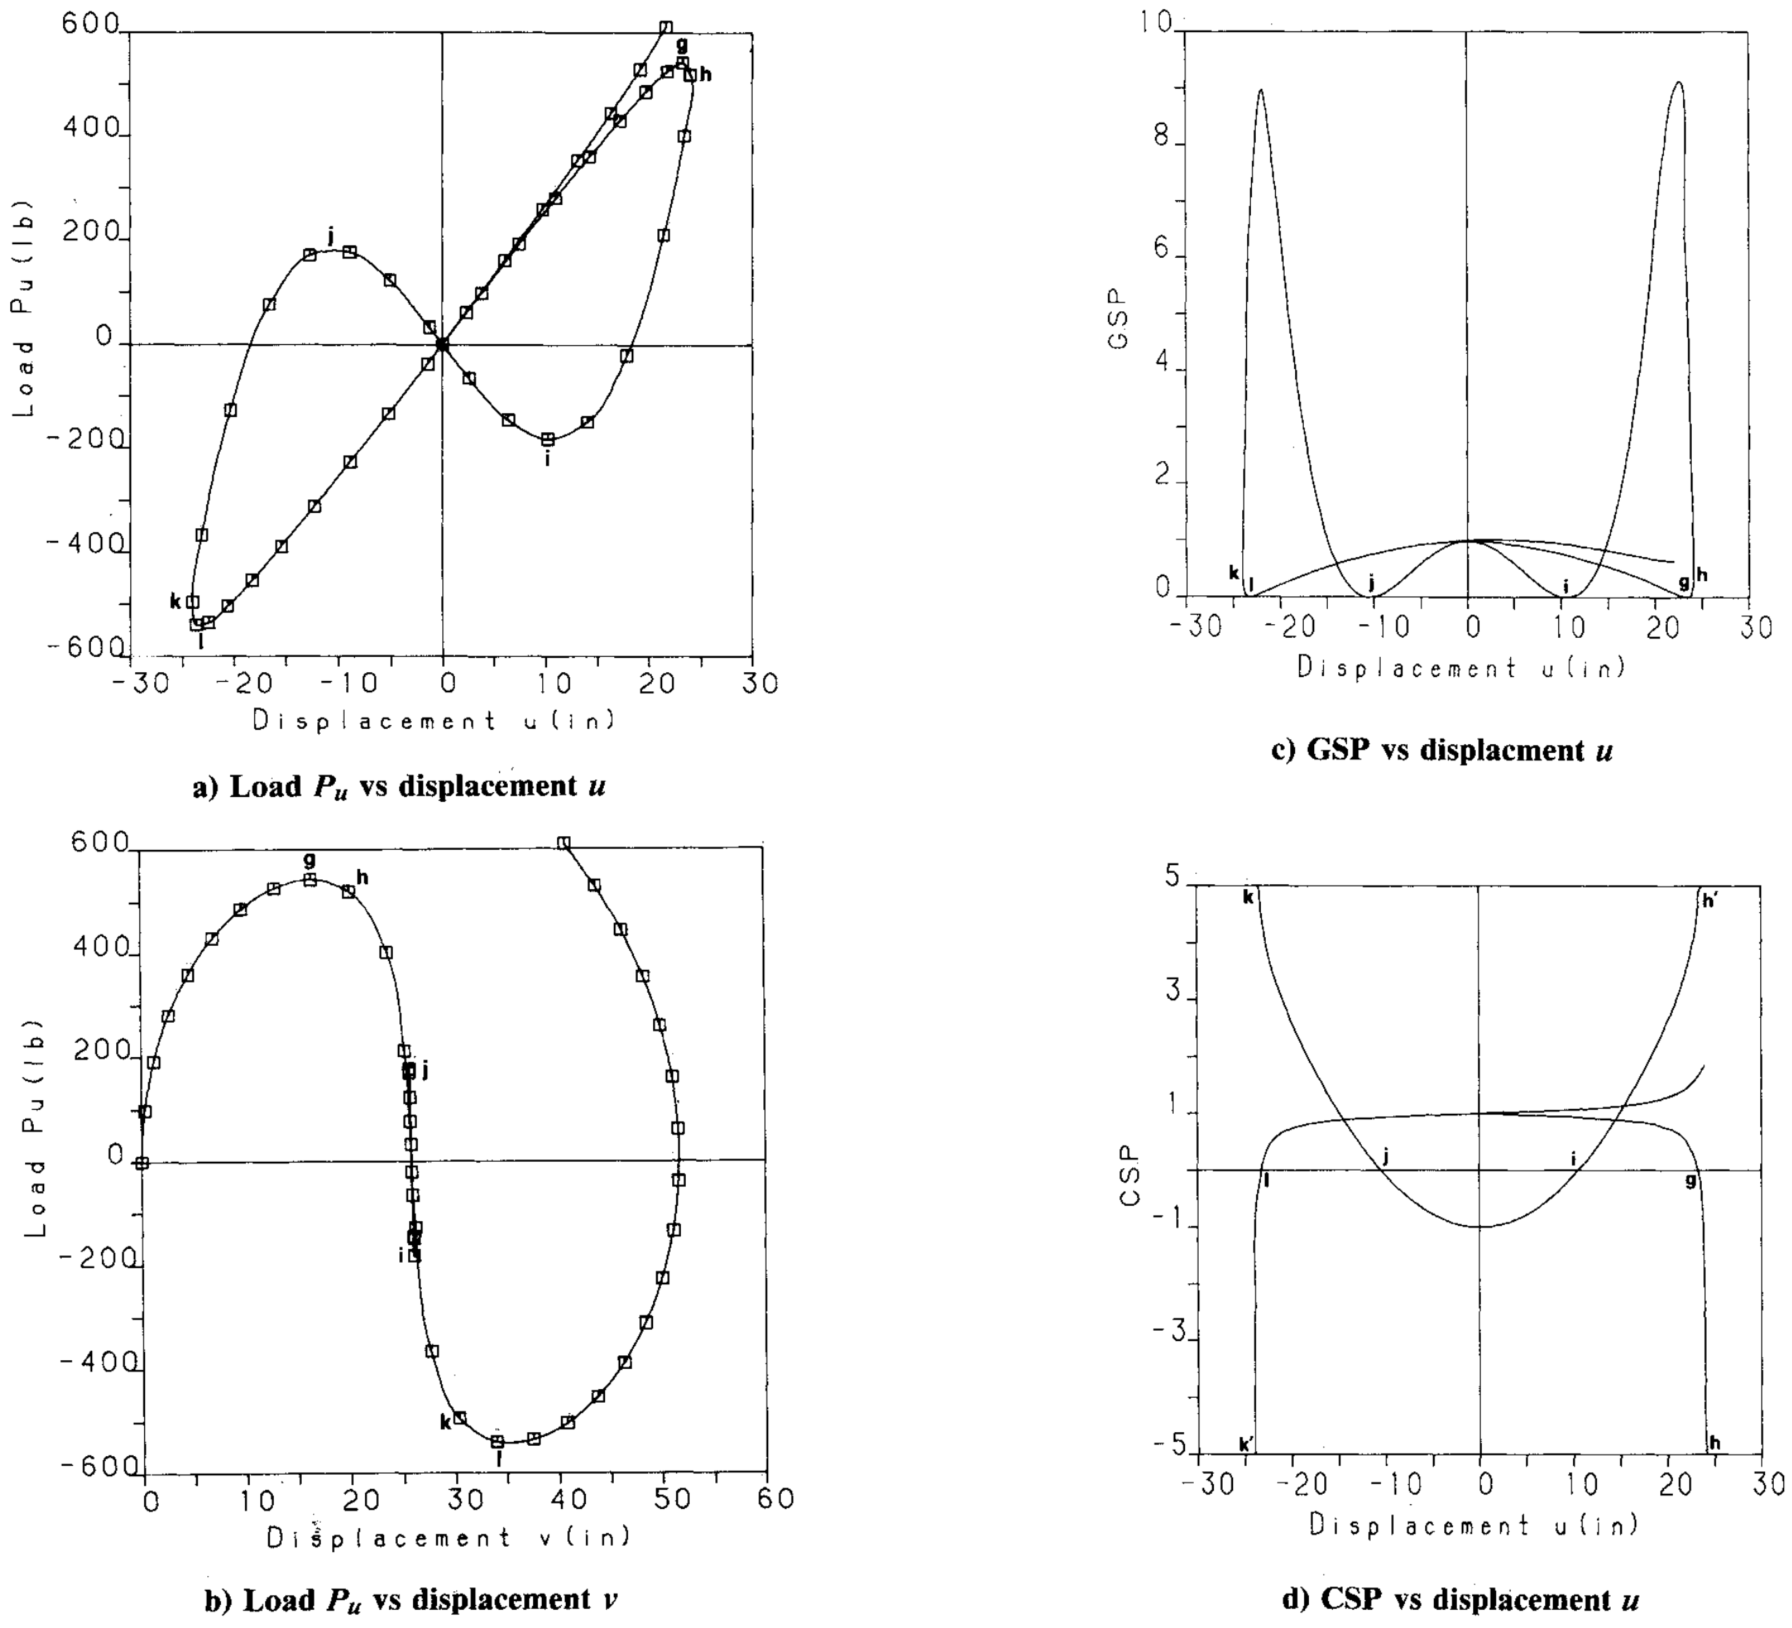
\includegraphics[
		width=0.95\textwidth
	]{figuras/TP10-ex1_result2.png}
	\caption*{Fonte: Adaptado de YANG, Y. -B.; SHIEH, M. -S. (1990)}
	\label{fig:TP10-ex1_result2}
\end{figure}

\textbf{Exemplo 2 -- Arco circular bi-articulado}

\begin{figure}[H]
	\centering
	\caption{Treliça de dois membros.}
	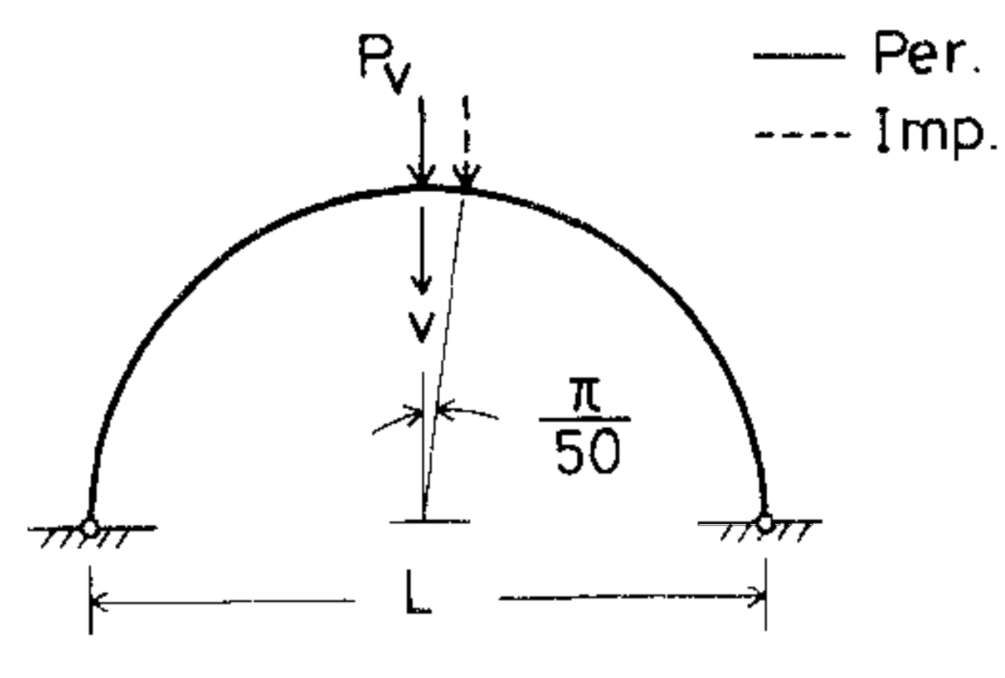
\includegraphics[
		width=0.4\textwidth
	]{figuras/TP10-ex2.png}
	\caption*{Fonte: Adaptado de YANG, Y. -B.; SHIEH, M. -S. (1990)}
	\label{fig:TP10-ex2}
\end{figure}

Representado por 26 elementos de viga
plana, o arco é submetido a carregamentos simétrico e assimétrico (com imperfeição de
posição). Os gráficos de carga-deslocamento exibem respostas de pós-flambagem com múltiplas
oscilações, demonstrando a capacidade do método de acompanhar trajetórias complexas com
grandes deformações.

\begin{figure}[H]
	\centering
	\caption{Resultados gerais do Exemplo 2.}
	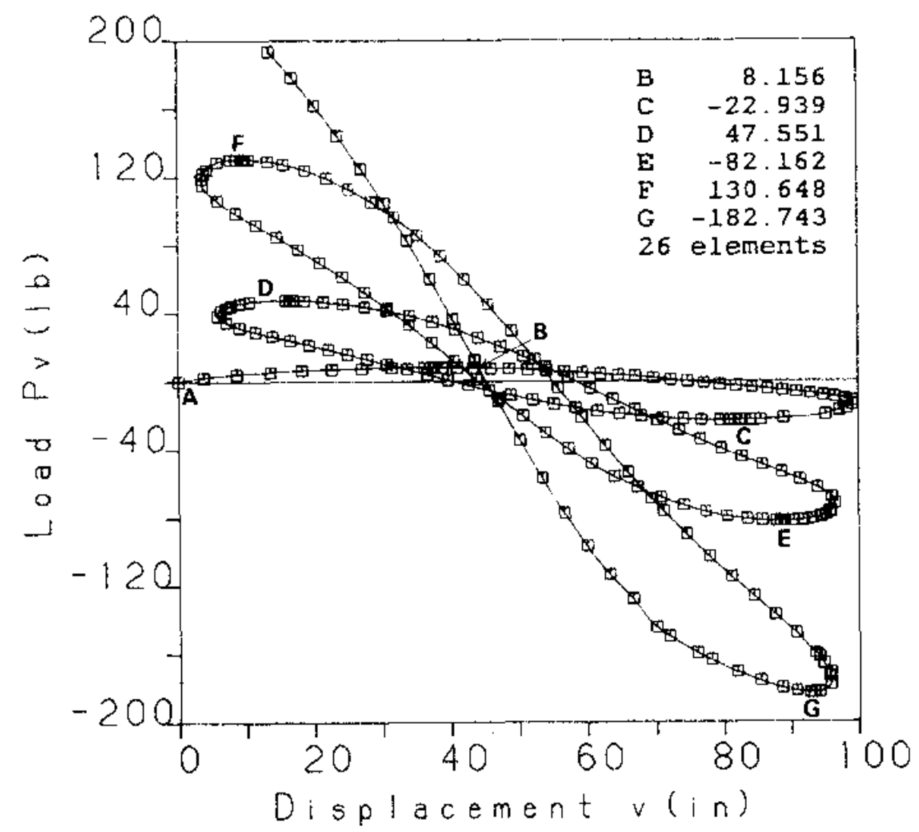
\includegraphics[
		width=0.6\textwidth
	]{figuras/TP10-ex2_result.png}
	\caption*{Fonte: Adaptado de YANG, Y. -B.; SHIEH, M. -S. (1990)}
	\label{fig:TP10-ex2_result}
\end{figure}

\subsection*{Conclusões}

O Método de Controle de Deslocamento Generalizado satisfaz simultaneamente os três
critérios fundamentais para métodos de solução não-linear:

\begin{enumerate}
	\item[(i)]   \textbf{estabilidade numérica} nas proximidades de pontos limite e de
	\textit{snap-back}, mantendo $\lambda^i_j$ e $\{u\}^i_j$ limitados;
	\item[(ii)]  \textbf{ajuste automático do tamanho dos passos} por meio do GSP, que
	reflete diretamente a variação de rigidez da estrutura ao longo da trajetória;
	\item[(iii)] \textbf{capacidade autoadaptativa} de inversão da direção de carregamento,
	usando o sinal do GSP como indicador exclusivo dos pontos limite. O método pode ser
	implementado diretamente em programas de elementos finitos de propósito geral para
	análise não-linear geométrica.
\end{enumerate}

\end{textocaixa}